\documentclass[11pt]{article}
\newcommand{\numpy}{{\tt numpy}}    % tt font for numpy
\usepackage[margin=.9in]{geometry}
\usepackage{hyperref}
\usepackage{graphicx}
\hypersetup{
    colorlinks=true,
    linkcolor=cyan,
    filecolor=magenta,      
    urlcolor=blue,
}

\begin{document}

$$\mbox{\Large \textbf {CS 111 (S19): Homework 6}}$$
$$\mbox{\textbf {Due by 6:00 PM, Wednesday, May 29}}$$
$$\mbox{\textbf {NAME and PERM ID No.:} Chen Li, 5468137 (replace with yours)}$$
$$\mbox{\textbf {UCSB EMAIL:} chenli@ucsb.edu (replace with yours)}$$


This is the comparison between PG1 and PG2 on EG1\\
$$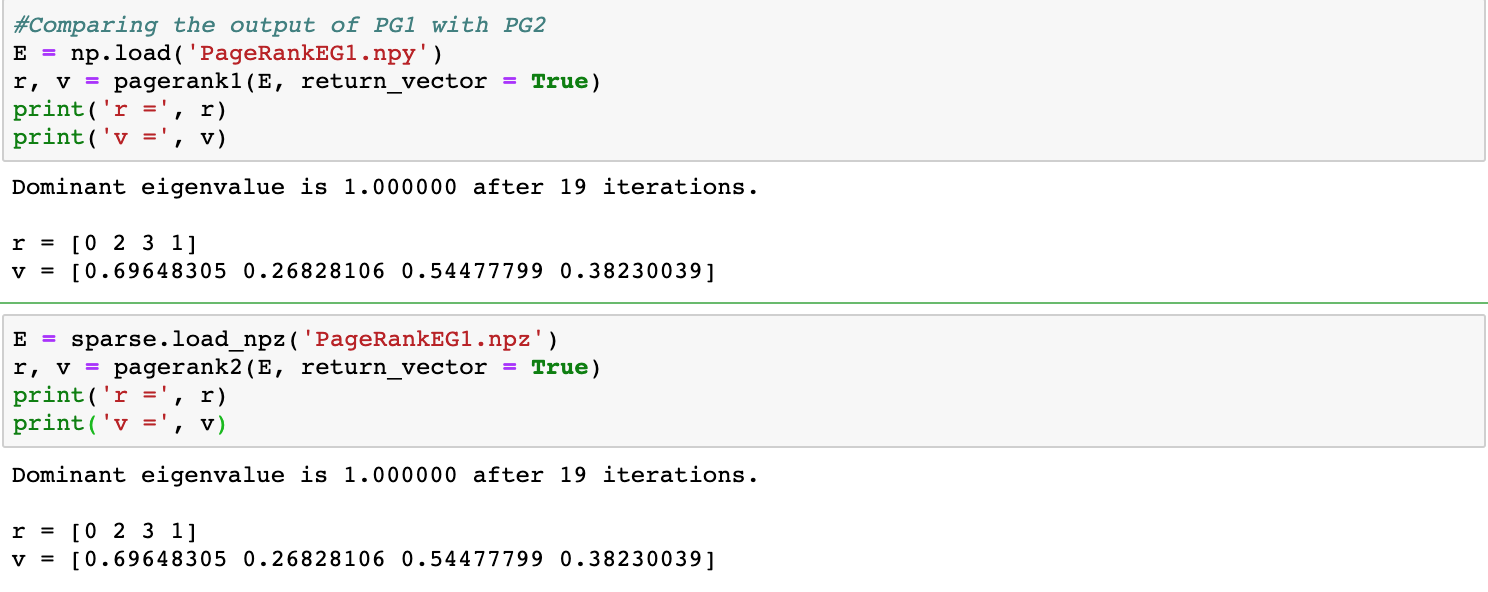
\includegraphics[scale = 0.5]{h6eg1}$$\\
\\This is the comparison between PG1 and PG2 on EG3, on my machine, it took 15.7ms  to run PG1 and took 12.6ms to run PG2. PG2 is slightly faster \\
$$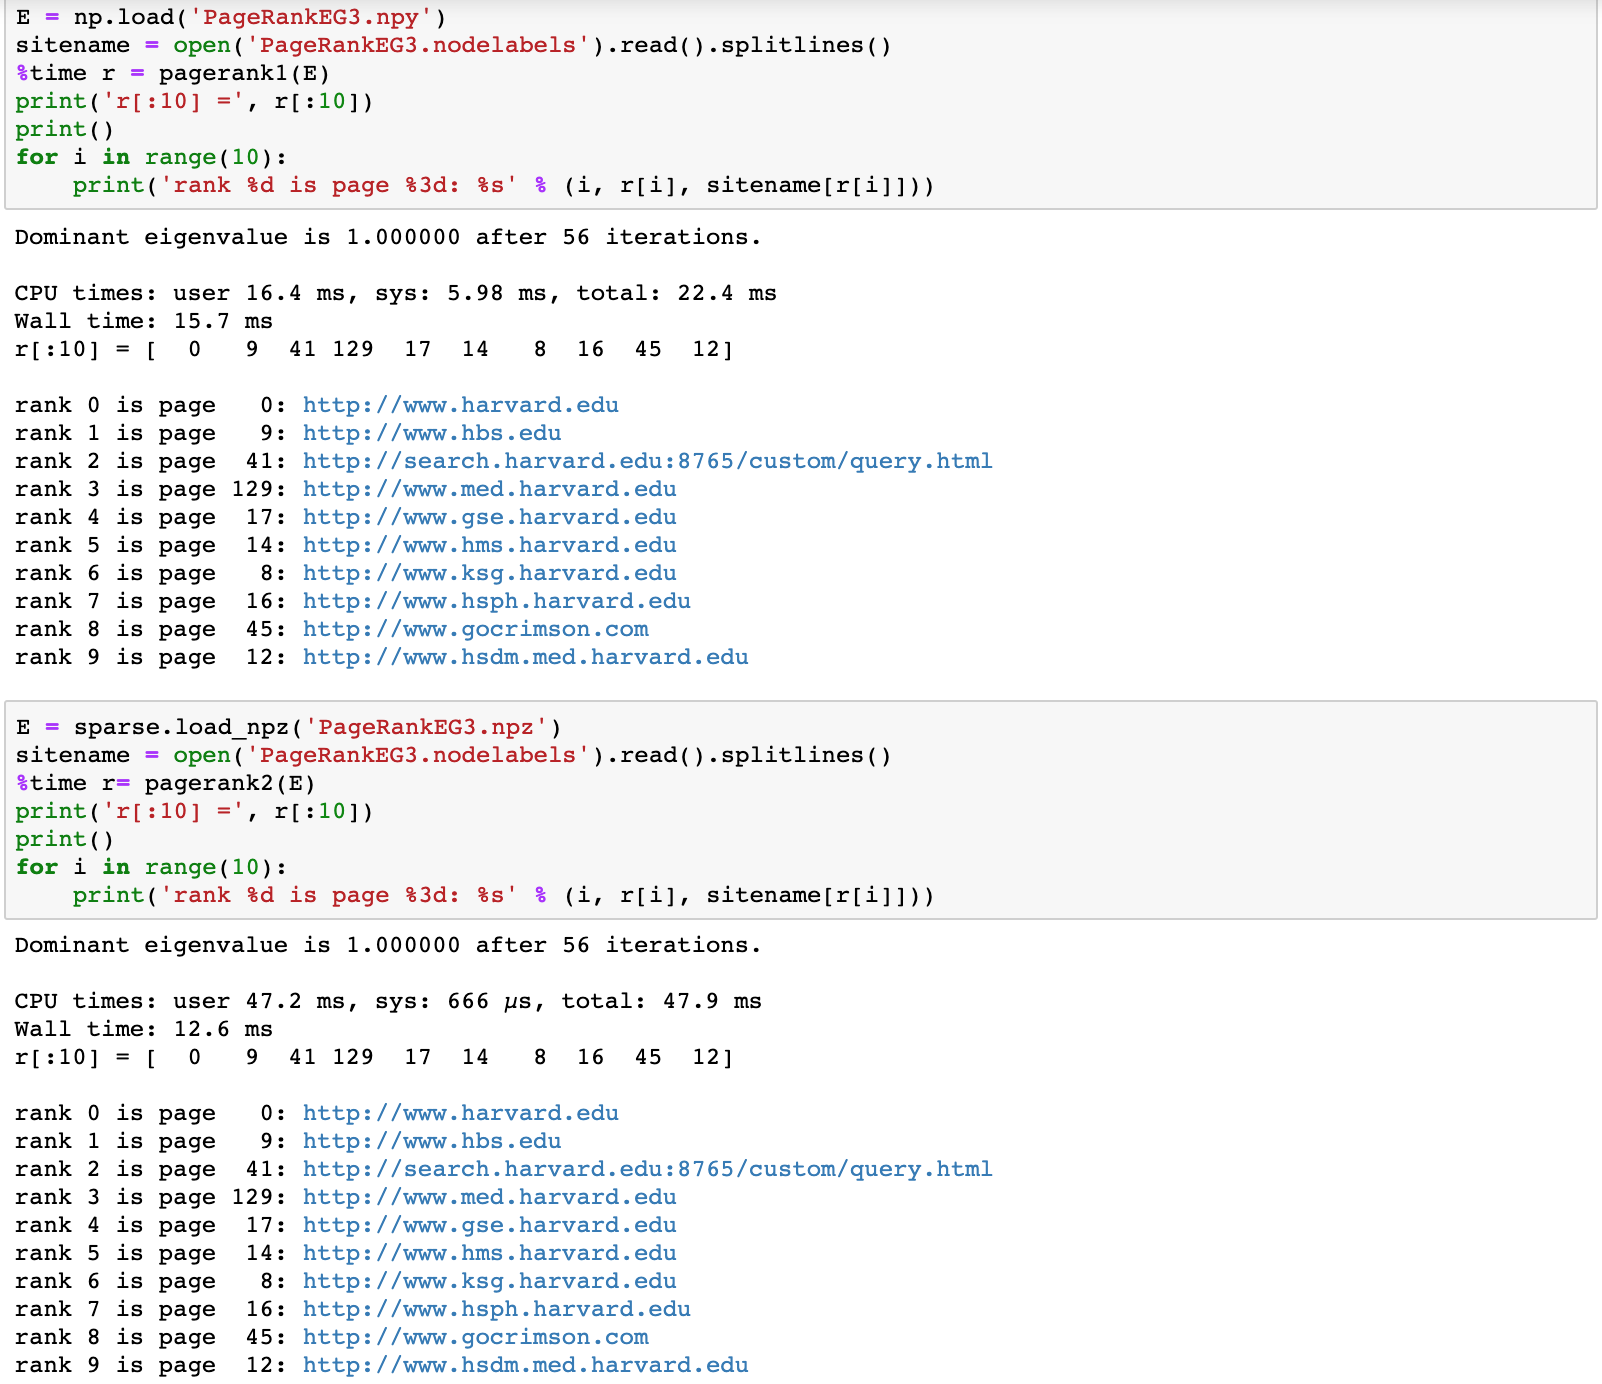
\includegraphics[scale = 0.4]{h6eg3.png}$$
\newpage
It took 10.4 second to run PG2 and only 5.42 second to run spla.eigs. max is 0.11427415903139658 and min is 0.00013008094286810808
$$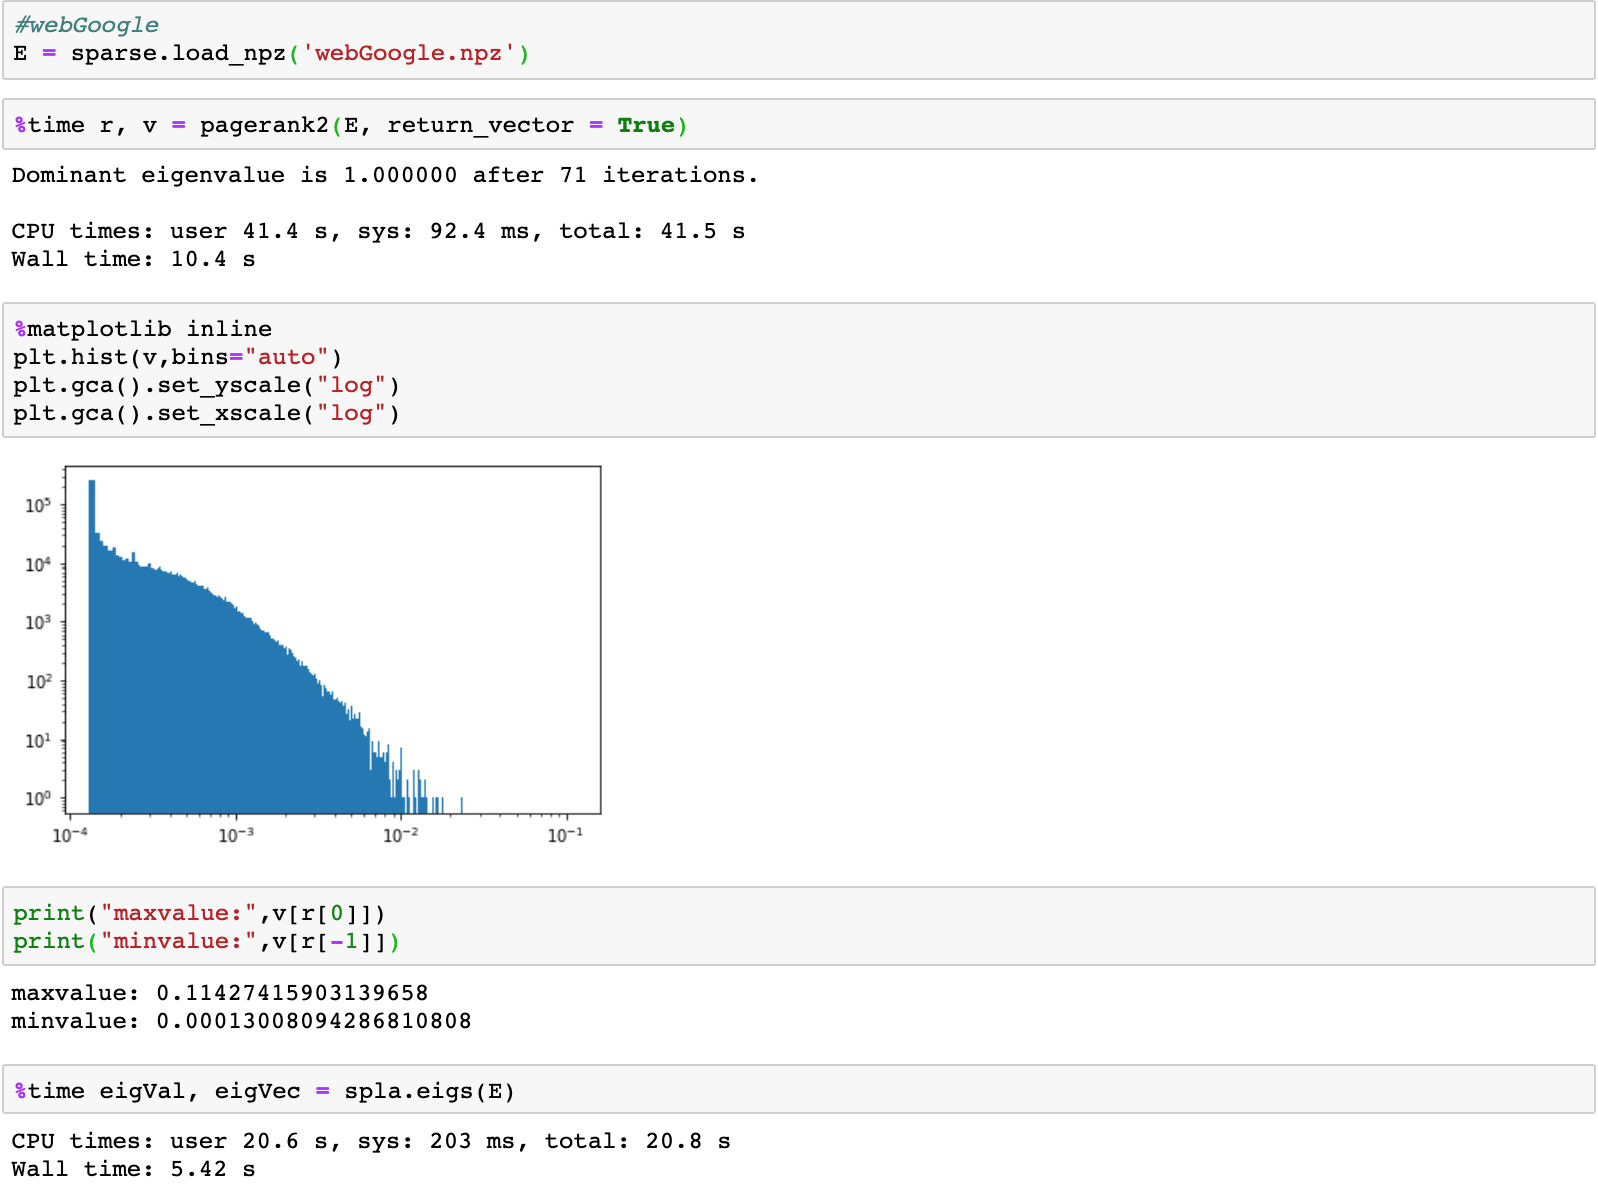
\includegraphics[scale = 0.6]{webGoogle.png}$$



\end{document}
